\documentclass[preprint,3p,times,twocolumn]{elsarticle}
\usepackage{graphicx}
\usepackage{color}
\usepackage{amssymb}
\usepackage{amsmath}
\usepackage{multirow}
\usepackage{multicol}
\usepackage{array}
\usepackage{rotating,capt-of}
\usepackage[small]{caption}
\usepackage{booktabs}
\usepackage{float} % for placing figures where i want
\usepackage{afterpage}
\usepackage{epsfig, a4wide}

\newcommand{\myparagraph}[1]{
  \paragraph*{\normalfont\itshape #1}\hspace{5pt}}

% strange snos
\definecolor{purple}{RGB}{180,90,200}
\definecolor{dgreen}{RGB}{0,160,0}
\definecolor{turquoise}{RGB}{0,180,140}
\renewcommand\dblfloatpagefraction{0.03}
\renewcommand\topfraction{.95}
\renewcommand\bottomfraction{.95}
\renewcommand\textfraction{.05}
\renewcommand\floatpagefraction{.95}
\renewcommand\dbltopfraction{.95}
\renewcommand\dblfloatpagefraction{.95}
\newcommand{\TODO}[1] {\begingroup\color{red}#1\endgroup}
\newcommand{\SC}[1] {\begingroup\color{purple}#1\endgroup}
\newcommand{\ACC}[1]{\emph{\textbf{#1}}}
\newcommand{\s}[1]{\begin{tiny}#1\end{tiny}}
\newcommand{\url}[1]{\texttt{https://\small #1}}
\newcommand{\maxentscan}{\texttt{MaxEntScan}}
\newcommand{\NEW}[1]{\begingroup\color{black}#1\endgroup}

%% programs
\newcommand{\spps}{\texttt{SPPS}}
\newcommand{\tri}{\texttt{TRI\_tool}}
\newcommand{\lr}{\texttt{LR\_PPI}}

%% databases
\newcommand{\ncbi}{\texttt{NCBI}}
\newcommand{\nega}{\texttt{Negatome Database}}
\newcommand{\kups}{\texttt{KUPS}}

%\newcommand{\tool}{\texttt{rfPRO}}
%\newcommand{\tool}{\texttt{jackProt}}
\newcommand{\toolblank}{\texttt{ProteinPrompt}}
\newcommand{\tool}{\toolblank\hspace{2pt}}
\newcommand{\website}{\url{proteinformatics.org/\tool}}

\newcommand{\Hsa}{\emph{Homo sapiens}}
\newcommand{\hsa}{\emph{H.sapiens}}

\journal{Preprint}

\DeclareCaptionLabelFormat{simplesupp}{#1~S#2} % new caption format with Sxx

\begin{document}

\begin{frontmatter}
   
\title{\tool: fast and accurate prediction of Protein-Protein-Interactions}

\author[LEI,IMT]{Sebastian Canzler\corref{cor1}}
\ead{sebastian@bioinf.uni-leipzig.de}
\author[PHY,IMT]{Ren\'{e} Staritzbichler\corref{cor1}}
\ead{rene.staritzbichler@medizin.uni-leipzig.de}


\address[LEI]{Bioinformatics Group, Department of Computer Science,
  University of Leipzig,
  H{\"a}rtelstra{\ss}e 16-18, 04107 Leipzig, Germany
}
\address[PHY]{ProteinFormatics Group, Institute of Medical Physics and Biophysics, University of Leipzig,
  H{\"a}rtelstra{\ss}e 16-18, 04107 Leipzig, Germany.}

\address[IMT]{Immuthera GmbH, L{\"o}{\ss}niger Stra{\ss}e 16, 04275 Leipzig, Germany.}


%\cortext[jfa]{Joint first authors}
\cortext[cor1]{Corresponding author}

% --------------------------------------------------------------------------- %
 

\begin{abstract}

  Here, we present \tool, a precise machine learning method for the calculation of protein-protein interactions.
  Learning methods depend crucially on both size and quality of datasets used for training and testing.
  Starting point of \tool was therefore the collection of a comprehensive dataset from basically all available sources.
  In turn, a very thorough filtering was imperative.
  The actual keystep is the transformation of the original sequence data into a representation that enables the learning algorithm to understand the underlying patterns that lead to binding versus non-binding.
   \tool exploits the random forest algorithm using auto-correlation of seven amino-acid scales.
   Based on this combination, \tool is reaching an area under curve of 0.95, which is far above any other publicly available tool. 
  
  \tool  is accessible online as a webserver:
  \website
  The server allows  scanning the human proteasome for potential binding partners of the query in unprecedent accurracy.
  A scan through the entire human proteasome is performed within minutes.  
  

\end{abstract}

\begin{keyword}
  protein-protein-interaction, machine learning, random forest
\end{keyword}

\end{frontmatter}

% --------------------------------------------------------------------------- %

\section{Introduction}

Interacting proteins are among the keyplayers of biology. The driving
force of molecular networks are protein interactions rather than
single protein components, accomplishing their individual functions
\cite{Pawson:2004}. Biological processes, such as cellular
organization, communication, regulation of transcription and
translation, or immune responses require various proteins to interact
and work together to function appropriately. The experimental
identification of interacting proteins is highly expensive and time
consuming.

Many biochemical and biophysical methods for research and medical diagnostics are based on protein-binding:
ELISA,
gel electrophoresis, immunoblot, florescence anisotropy, FRET,
Cross-linking with mass spectrometry. For high-throughput-screening of
large libraries there are techniques such as phage display. 

A reliable \textit{in silico} prediction of protein-protein
interactions (PPI) will therefore shed more light on biological and
pharmacological responses and pathways. Computations may complement
and guide biochemical assays. However, explicit molecular dynamics or
docking approaches require structural detail, which is often out of
reach. Even if structural knowledge is available, these methods are
computational highly expensive and therefore are not applicable for
scanning libraries of candidates. 

Both when structural insight is lacking and when speed is crucial,
other methods need to be applied. Non structure based computational
approaches of identifying potential PPIs are generally based on an
extensive set of known protein-protein interactions, information about
cellular localization, amino acid sequences, or secondary structures.

Such methods may include phylogenetic trees \cite{Pazos:2001},
phylogenetic profiles \cite{Barker:2005}, network-based methods
\cite{Yook:2004, Clauset:2008}. In recent years, the more
sophisticated approach of combining distinct prediction methods has
been applied, e.g., \texttt{STRING} \cite{Szklarczyk:2011} or
\texttt{PIPS} \cite{McDowall:2009}.

Nevertheless, different proteome-wide prediction methods have shown
that knowledge of the amino acid sequence alone may be sufficient to
identify novel, functional protein-protein interactions
\cite{Martin:2005, Shen:2007}. Due to its prominent and major
advantages like simplicity, rapidity, and generality, this kind of
prediction method became increasingly widespread over the last years
\cite{Ofran:2003, Betel:2007, Liu:2012, Perovic:2017,
  Pan:2010}. Overall, Biology has seen a massive raise in applications
of artificial intelligence and deep learning in the recent years
\cite{Ching:2018}.

In this paper, we present a sequence-based web-tool for predicting
PPIs that outperforms all other currently available methods distinctively.
The predictive power was boosted by a rigorous fine-tuning
of the machine learning key-elements, such as
dataset generation and the design of the feature vector.
Auto-correlation of hydrophobicities,
in conjunction with a random forest (RF) machine learning algorithm,
has lead to maximum accuracy.
Additionally to its outstanding quality, it is 
an extremely fast high-throughput
method.

Therefore, \tool (protein \textbf{pr}ediction \textbf{o}f \textbf{m}atching \textbf{p}ar\textbf{t}ners)
may serve as a reliable tool for identifying potential interaction partners from a database of
known proteins, and may thus help to identify the yet unknown
biological role of many proteins.


% --------------------------------------------------------------------------- %

\section{Materials and Methods}

To maximize the predictive power, it is pivotal to optimize each of
the key-elements, i.e., the calculation of the feature vector, the
collection of the training and testing data, and finally, the
selection and fine-tuning of the machine learning algorithm. 

For all aspects, many variations were tested. Here we focus on the
ones leading to the highest accuracy. 


\subsection{Feature vector calculation}
The feature vector calculation includes the extraction and
transformation of sequence-based information into a numerical vector
of constant size. Therefore, it is crucial to extract the properties
that are responsible for directing the protein-protein interaction. 

Each amino acid sequence of a protein-protein complex was transformed
into a sequence of numerical values representing seven
sequence-derived physicochemical properties, which include
hydrophobicity \cite{Eisenberg:1984, Koehler:2009}, hydropyhilicity
\cite{Hopp:1981}, volumes of side chains of amino acids
\cite{Krigbaum:1979}, polarity \cite{Grantham:1974}, polarizability
\cite{Charton:1982}, solvent-accessible surface area \cite{Rose:1985}
and net charge index of side chains of amino acids \cite{Zhou:2006}
for each residue in sequence. These scales are commonly applied in
protein interaction prediction \cite{Bock:2001} \cite{Bock:2003},
alignment \cite{Stamm:2013}, protein recognition \cite{Ding:2001},
protein structure prediction \cite{Durham:2009}, or the prediction of
protein functional families \cite{Cai:2003}. These applications
suggest that these properties significantly contribute to the
stability of the protein-protein complexes. Each of these amino acid
scales was normalized as follows: 

\begin{equation}
P'_{i} = (P_i - \overline{P}) / \sigma_P
\end{equation}

where $\overline{P}$ is the mean and $\sigma$ is the standard
deviation of the scale-based descriptor covering 20 amino acids,
respectively: 

\begin{equation}
\overline{P} = \sum^{20}_{i=1}P_i / 20
\end{equation}
 and 
\begin{equation}
\sigma_P = \sqrt{\frac{1}{20} \sum^{20}_{i=1}(P_i - \overline{P})^2}
\end{equation}

The subsequent transformation into suitable feature vectors using
auto-correlation (AC) works as follows: 

\begin{equation}
AC_{lag, j} = \frac {\frac{1}{n-lag} \sum^{n-lag}_{i=1} ( S_{i,j} - \overline{S_j}) (S_{i+lag,j} - \overline{S_j})} { \sigma_{S_j} * \sigma_{S_j} }
\end{equation}
with $S_j$ is the translated amino acid sequence using the normalized
scale-based descriptor $P'_j$ with $j = 1, 2, \dots, 7$ , $n$ is the
length of sequence S, and $lag = 1, 2, \dots, 30$  being the shift for
which the auto-correlation is being calculated. $\overline{S_j}$ and
$\sigma_{S_j}$ are the mean and standard deviation of the translated
sequence, respectively. Ding \cite{Ding:2016} showed that a maximal
$lag$ of less than 30 tends to lose useful information while the
larger values may induce noises. 

The number of AC values for each of the seven scales is 30. Finally
the feature vector describing a given amino acid sequence is produced
of 210 dimensions and for a pair of sequences, the feature space
contains 420 dimensions. 


\subsection{Collecting data-points}
In order to create comprehensive training and testing data we tried to
collect as many trustworthy PPI annotations as possible. We included
data from various sources such as \texttt{Database of Human
  Interacting Proteins}\footnote{http://dip.doe-mbi.ucla.edu/} (DIP)
\cite{Salwinski:2004}, \texttt{Human Protein Reference
  Database}\footnote{http://www.hprd.org/} (HPRD)
\cite{Keshava_Prasad:2009}, \texttt{Protein
  Database}\footnote{www.rcsb.org} (PDB) \cite{Berman:2000}, and the
\nega\footnote{http://mips.helmholtz-muenchen.de/proj/ppi/negatome/}
\cite{Blohm:2014}. We also included annotations retrieved from the
\kups \footnote{http://www.ittc.ku.edu/chenlab/kups/}   server
\cite{Chen:2011} which mainly incorporates PPIs from
\texttt{MINT}\footnote{https://mint.bio.uniroma2.it/}
\cite{Licata:2012} and
\texttt{IntAct}\footnote{https://www.ebi.ac.uk/intact/}
\cite{Orchard:2014}. In addition to the negative annotations collected
from the \nega, the \kups\ server generated negative data-points based
on the the following criteria: (1) proteins should be functional
dissimilar, (2) proteins should be localized in different cellular
compartments, and (3) proteins are part of non-interacting domains. 

After intense manual curation and mapping of different names describing
the exact same protein, we derived a total amount of 31.867 distinct
human proteins. For this set, 73.681 positive PPIs were collected
from the datasources previously mentioned. By means of \texttt{CD-hit}
\cite{Li:2006, Fu:2012}, we reduced this set to 41.844 positive
protein-protein pairs with at most 50\% sequence identity. For
negative pairs, we collected over 1.5 million unique protein-protein
pairs, from which we randomly selected a number of PPIs, that was
matching the size of the positive dataset.

Finally, our training dataset contains 36.750 positive and 36.750
negative PPIs, while our testing dataset contains 5094 positive and
5094 negative data-points. For further enhancement of the prediction
quality of \tool, we also incorporated inverse and reverse PPI
representations. Each protein-protein pair $AB$ is described in the
original and inverse (') direction, as well as in original and
reversed order. In the final dataset each annotated PPI is represented
in four distinct descriptions\footnote{Example pseudo-sequences: (ABCD,KLMN),
  (ABCD,NMLK), (KLMN,ABCD), (KLMN,DCBA)}: $AB$, $AB'$, $BA$, and
$BA'$. 

To verify the prediction quality of \tool, we compared our tool to
several other publicly available programs. As some of them are limited
in speed or upload capacity to their webserver, it was not
feasible to perform this test using our entire test dataset with more
than 10k datapoints. Instead, we randomly selected 495 positive and 473
negative pairs from our test set.

\subsection{Selection of learning method}
Plenty implementations of various learning algorithms are
available. By means of the \texttt{caret} R package \cite{Kuhn:2008},
the fine-tuning and comparison is relatively easy. We tested several
artificial neural network implementations, support vector machines and
tree-based methods. After electing the random forest approach as
performing best on our extensive testing and training datasets,
we moved to a Python-based implementation mainly
because of speed reasons.  

\subsection{Random forest classification}
Random forest (RF) is an algorithm, which uses an ensemble of
classification trees. Each classification tree is built by using a
bootstrap sample of training data, and each split candidate set is a
random subset of variables. RF uses both bagging (bootstrap
aggregation) and random variable selection for tree building. Each
classification tree is unpruned to obtain low-bias trees. The bagging
and random variable selection can cause low correlation of individual
trees. Therefore, RF has excellent performance in classification
tasks. 

We define a 420-dimensional feature vector $F=(x_1,x_2,
\dots,x_{420}$) as the input data of RF model. If the number of cases
in the training set is $N$, the sample is built by randomly choosing
$N$ cases from the original data, but with replacement. This sample
will be the training set for growing the tree. There are $M$ input
variables, a number $m \ll M$ is specified such that at each node, $m$
variables are selected at random out of $M$ and the best split on
these m is used to split the node. The value of $m$ is held constant
during the forest growing. Each tree is grown to the largest extent
possible without pruning. The final number of trees in the forest is
set to 750 due to run-time optimization. 




% --------------------------------------------------------------------------- %

\section{Results}

\subsection{Webserver implementation}

\tool is available online as webserver under: \website The basic usage
is as simple as providing an input sequence. By default \tool will
search our manualy curated database of human protein sequences
containing 31.867 proteins. Scanning the entire human database takes
approximately one minute. Other more extensive databases are provided
as well as additional service, e.g. mammalian, vertebrate, and
metazoan protein sets. Searching these databases takes considerably
longer. However, since \tool\ is trained and optimized
on human proteins, we cannot guarantee an equivalent prediction
quality for other organisms. 

The server is free for academic users. Providing an email is
optional.
%Results for anonymous users will be made accessible via a
%public search engine.
\tool\ was originally optimized for sequences with a minimum length of 16 AA.

%\TODO{Ist das in dem webserver so umgesetzt?
%
%There are two ranges of sequence lengths, for which \tool\ was
%optimized: 
%\begin{itemize}
%\item \TODO{? - ?} AA
%\item \TODO{? - ?} AA
%\end{itemize}
%}

The sequence length of the uploaded proteins is detected automatically. When the user provides
sequences shorter than 16aa, a warning is thrown,
the calculation is performed nonetheless.
%\TODO{Check}

As output a ranked and scored list of proteins from the database is
returned. By default it is truncated after the first 100 top
hits. This can be adjusted on the webform. 

%\TODO{ screenshots}

\subsection{Performance}
\label{performance}

Based on our test set of 5094 positive and 5094 negative cases
(binders vs. non-binders), we plot the receiver operation
characteristics (ROC) curve, see Figure \ref{fig:roc}.
These allow not only to estimate the overall quality of the predictions, but also
gives a visual overview over the relationship between true and false
positives. This allows to select a useful threshold and thus a
finetuning of sensitivity versus specificity.

An ideal signal would lead to a plot with rectangular shape
with an area under the curve (AUC) of 1. The other extreme, pure noise, would be a crossing
line with an AUC of 0.5.

Our method reaches an AUC of 0.95,
specificity: 0.88,
sensitivity: 0.87,
accuracy: 0.88.

Currently, our method balances specificity and sensitivity to avoid an
unwanted bias in different applications.
% \TODO{(is this the best solution for the server?)} 

\begin{figure}[t]
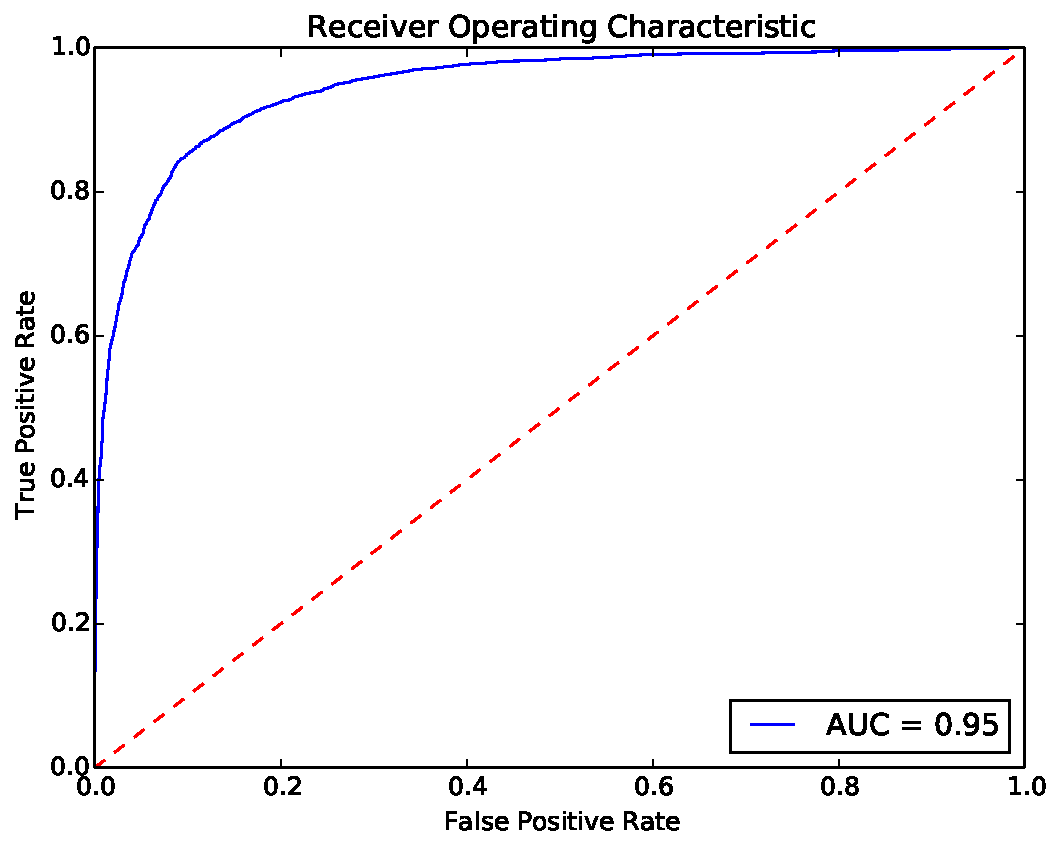
\includegraphics[width=0.5\textwidth]{img/meta_final_roc.pdf}
\caption{Performance of \tool tested on the whole test dataset
  containing over 10.000 PPIs.}
\label{fig:roc}
\end{figure} 



\subsection{Comparison to other tools}

To verify our achievements, we compared our program against publicly
available tools such as \spps\ \cite{Liu:2012}, \tri\
\cite{Perovic:2017}, and \lr\ \cite{Pan:2010}. Therefore, we used the
diminished test dataset, as described in the Methods section. 

Since we re-evaluated \tool on the dimished testset, to ensure
comparability, the results are somewhat different compared to the
whole testing data set. 

\begin{figure}
  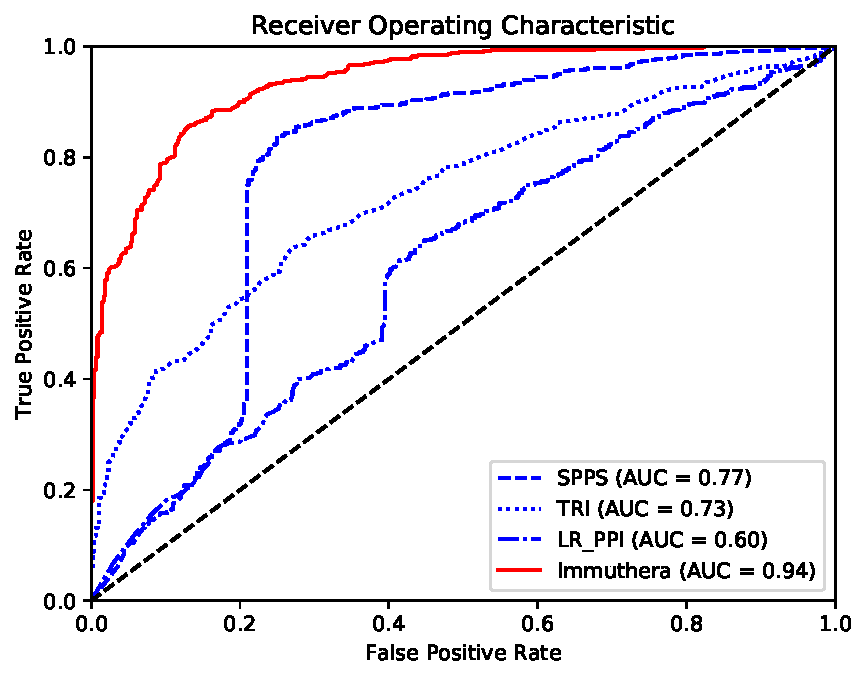
\includegraphics[width=0.5\textwidth]{img/comparison_roc.pdf}
  \caption{Comparison of ROC-curves between \tool, \spps, \tri, \lr\ 
    using the diminished test dataset that included 968
    protein-protein pairs.}
  \label{fig:comparison}
\end{figure}

%\begin{figure*}
%  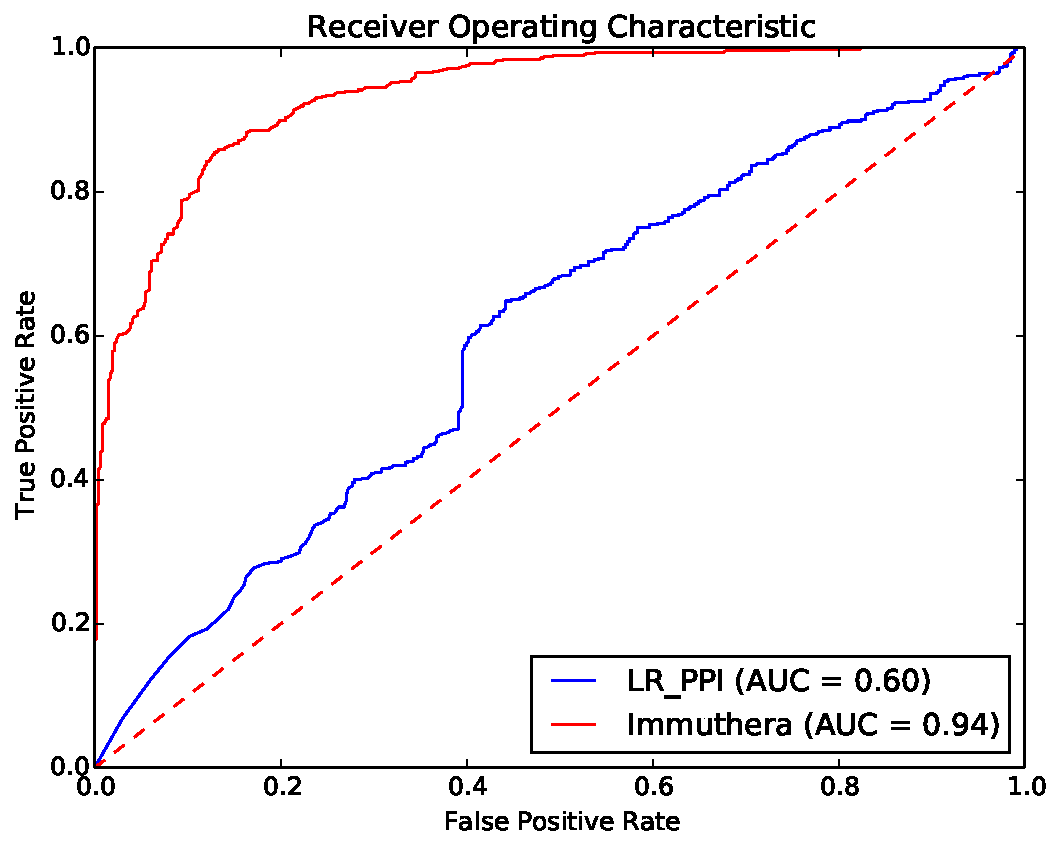
\includegraphics[width=200pt]{img/LR_PPI_roc.pdf}
%  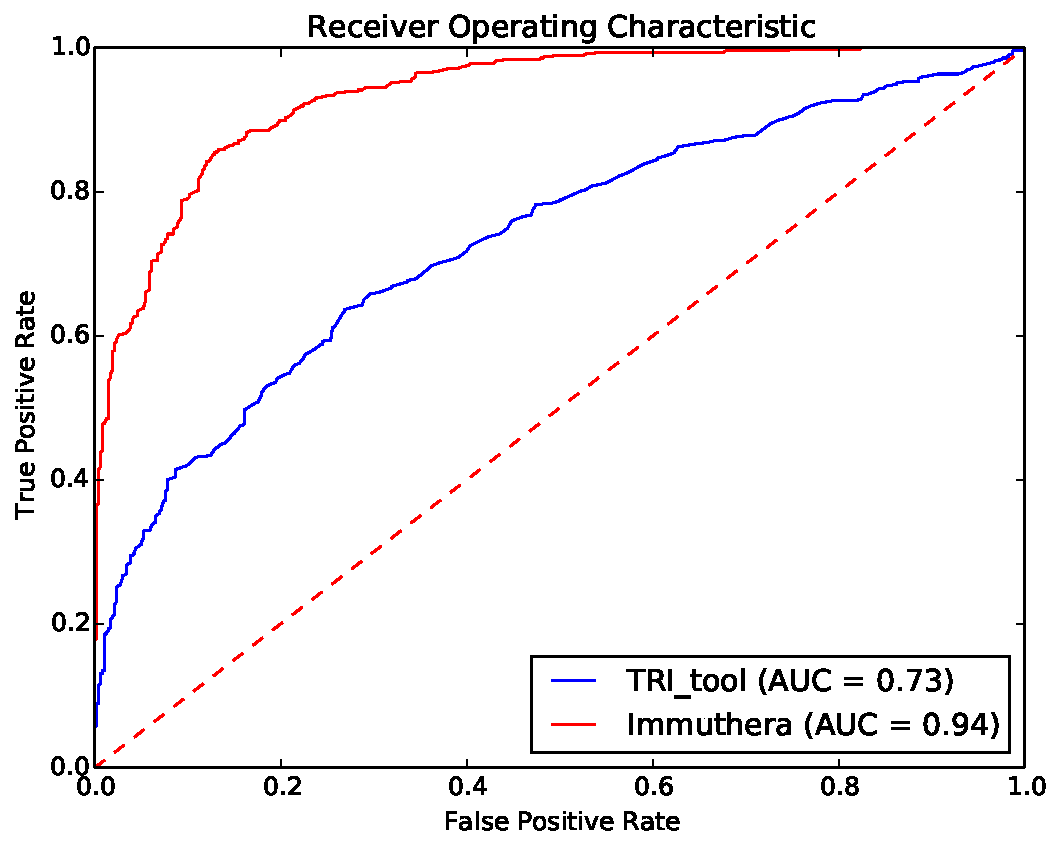
\includegraphics[width=200pt]{img/TRI_tool_roc.pdf} \\
%
%  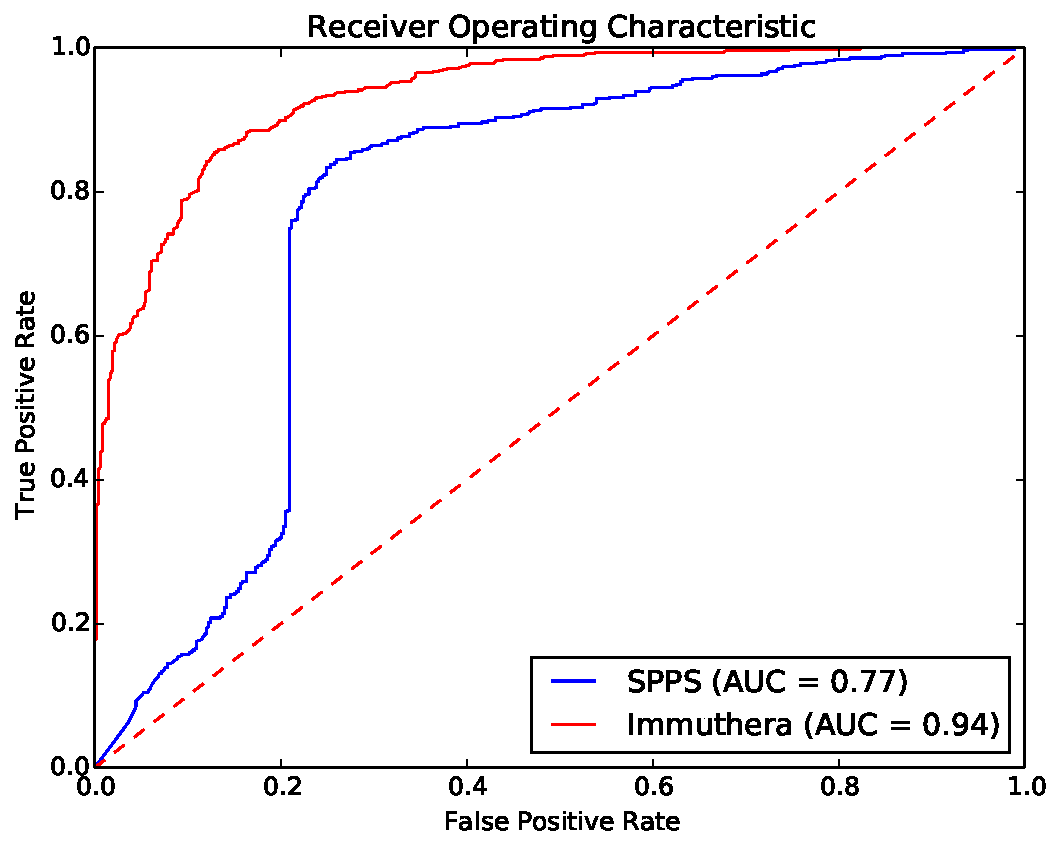
\includegraphics[width=200pt]{img/SPPS_roc.pdf}
%  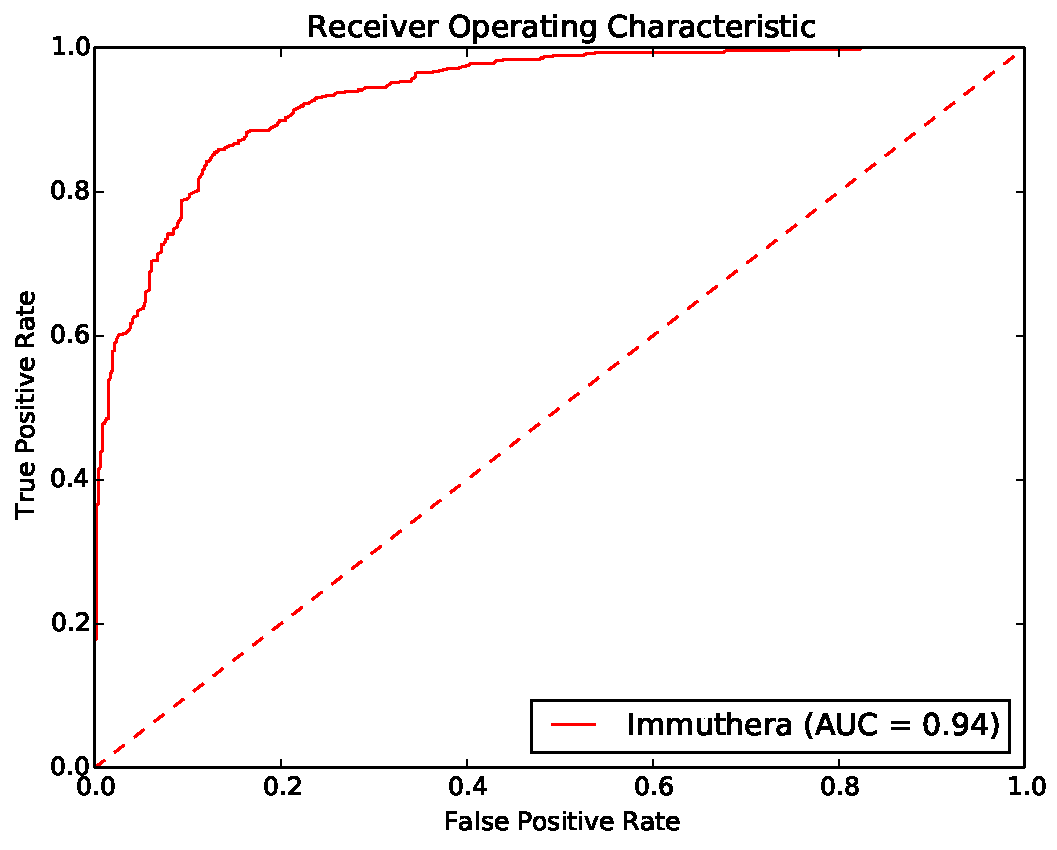
\includegraphics[width=200pt]{img/meta_roc.pdf}
%  \caption{Comparison of \tool to }
%  \label{fig:comparison}
%\end{figure*} 


%\begin{table*}
%\begin{tabular}{|c |c | c |}
%\hline
%Method  & Actual versus predicted & Quality \\
%\hline
%\tool  & \begin{tabular}{|c|c|c|} \firsthline  &  binder & non-binder \\ \hline binder: & 417 & 78 \\ \hline non-binder: & 58 & 415 \\ \hline \end{tabular} & \begin{tabular}{c} AUC: 0.94 \\ Spec.: 0.88 \\ Sens.: 0.84 \\ Acc.: 0.86 \end{tabular} \\
%\hline
%SPPS   & \begin{tabular}{|c|c|c|} \firsthline  &  binder & non-binder \\ \hline binder: & 474 & 21 \\ \hline non-binder: & 312 & 161 \\ \hline \end{tabular} & \begin{tabular}{c} AUC: 0.77 \\ Spec.: 0.34 \\ Sens.: 0.96 \\ Acc.: 0.66 \end{tabular} \\
%\hline
%TRI\_tool  & \begin{tabular}{|c|c|c|} \firsthline  &  binder & non-binder \\ \hline binder: & 158 & 337 \\ \hline non-binder: & 25 & 448 \\ \hline \end{tabular} & \begin{tabular}{c} AUC: 0.73 \\ Spec.: 0.95 \\ Sens.: 0.32 \\ Acc.: 0.63 \end{tabular} \\
%\hline
%LR\_PI  & \begin{tabular}{|c|c|c|} \firsthline  &  binder & non-binder \\ \hline binder: & 451 & 44 \\ \hline non-binder: & 398 & 75 \\ \hline \end{tabular} & \begin{tabular}{c} AUC: 0.60 \\ Spec.: 0.16 \\ Sens.: 0.91 \\ Acc.: 0.53 \end{tabular} \\
%\hline
%\end{tabular}
%\caption{ Quality measures of \tool, compared to other tools}
%\label{table:comparison}
%\end{table*}


\begin{table}
\begin{tabular}{|l |c | c | c | c |}
  \hline
  Tool  & AUC & Spec. & Sens. & Acc. \\
  \hline
  \tool  & 0.94 & 0.88 & 0.84 &  0.86 \\
  \hline
  \spps\  & 0.77 & 0.34 & 0.96 & 0.66 \\
  \hline
  \tri\  & 0.73 & 0.95 & 0.32 & 0.63 \\
  \hline
  \lr\  & 0.60 & 0.16 & 0.91 & 0.53  \\
  \hline
\end{tabular}
\caption{ Quality measures of \tool, compared to other publicly
  available tools, such as \spps\ \cite{Liu:2012}, \tri\
  \cite{Perovic:2017}, and \lr\ \cite{Pan:2010}.
  Listed are area under curve (AUC), specificity, sensitivity and accuracy.}

\label{table:comparison}
\end{table}

The results shown in Table \ref{table:comparison} and the ROC plot in
Figure \ref{fig:comparison} suggest that \tool clearly outperforms all
three competitors. \tool is furthermore the only tool that finds a
balance between sensitivity and specificity. \spps\ and \lr\ show an
excellent sensitivity of 0.96 and 0.91, however, their
specificity is rather poor with 0.34 and 0.16, respectively. \tri\ on
the other hand shows a massive bias towards specificity, 0.95 compared
to 0.32 .
Additionally, the overall prediction accuracy and the area under the curve are significantly higher.
Accuracy: 0.86 versus 0.66 (\spps), 0.63 (\tri).
AUC: 0.53 (\lr) and 0.94 versus 0.77 (\spps), 0.73 (\tri), and 0.60 (\lr), respectively.


\section{Discussion}

The direct comparison with other available tools prooved the
outstanding quality of \tool. Beside its high accurracy, \tool is the
only tool allowing to scan the entire human proteasome. This makes
\tool both the fastest and most accurate method available. We provide
full access via a webinterface: \website

After an exhaustive optimization of: i) the learning algorithm, ii)
the contact database, and iii) the representation of the binding
sequences, we identified a random forest using autcorrelation on seven
residue scales as the ideal combination.

The collection of an extensive database with little redundancy was crucial
and required several iterations of manual curation of the test and training datasets.
The diversity posed hard challenges to the learning
- it would have been easy to reach even higher accuracy values by omitting parts of our dataset.
However, this turned \tool into a broadly applicable tool.

In our next steps we will extend \tool to predict also the binding of short peptides to protein receptors, specifically to those of the GPCR family.
We furthermore intend to expand \tool towards antibody-protein binding.
Initial tests have shown, that the methods described in this paper are not directly applicable to this important class of protein interactions - which is easily understood, as the antibody binding mode via 3 very short loop segments does not reflect the general protein binding modes, covered currently by \toolblank. \TODO{ -- eher kritischer abschnitt, ist das sinnvoll?}

Based on our extensive tests, we expect
\tool to be beneficial for the understanding of complex networks of protein-protein interactions,
which are the basis for a broad range of mechanisms in biology.



%\begin{itemize}
% \item why is our tool better than the others?
% \item random forest approach
% \item far more datapoints in training data sets
% \item focusing on most important amino acid scales
%\item inverse reverse included
%\item trained on human proteins
%\item scan against nearly all annotated human proteins that are available
%\item comprehensive name mapping between different human protein databases
% \end{itemize}


% --------------------------------------------------------------------------- %

\section*{Acknowledgments}

This work was funded by the S\"achsische Aufbaubank (SAB).
Johanna Tiemann, Peter Hildebrand and Thorsten Kaiser for proofreading.
The universe for all the cookies.

%\stoptext

\bibliographystyle{unsrt}
\bibliography{ppi_prediction}

\end{document}


